% intro.tex

\chapter{介绍}
\label{ch:intro}

长久以来,发明家们梦想着创造会思考的机器。这种愿望至少可以追溯到古希腊时代。神话
人物皮格马利翁、代达罗斯和赫菲斯托斯都可以被理解为传说中的发明家,而伽拉泰亚、塔
罗斯和潘多拉都可以被视为是人工生
命\citep{ovid2004metamorphoses,sparkes1996red,1997works}。

当可编程计算机最初被设想时~——~在它被建造的超过一百年前~——~人们就想知道它们是否可
能变得智能\citep{Lovelace1842}。今天,\emph{\gls{ai} (AI)} 是一个茁壮成长的领域,
有着许多实际应用和活跃的研究课题。我们期待智能软件来自动化日常的劳动,理解语音或
图像,进行医学诊断和支持基础科学研究。

在\gls*{ai}早期,这个领域快速处理和解决一些问题,这些问题对人类脑力来说是困难的,
但对计算机来说则相对直接~——~这些问题可以通过一份有条理的、以数学规则的列表形式来
描述。\gls*{ai}的真正的挑战是解决那些容易被人执行,但是难于规范描述的任务~——~那些
我们凭直觉不假思索就能解决的问题,例如识别语音中的单词或者图像中的人脸。

这本书是关于这些更直观的问题的一个解决方案。这个解决方案是让计算机从经验中学习,
并以概念层次的形式理解这个世界,其中的每一个概念以和它相联系的、更简单的概念形式
定义。通过从经验中收集知识,这种方法避免了需要人类操作者规范地去指定计算机需要的
所有知识。概念的层次结构允许计算机通过建立更简单的概念来学习复杂的概念。如果我们
绘制一个图,显示这些概念是如何建立在彼此之上的,这幅图会很深,有许多层。因为这个
原因,我们称这种人工智能的方法为\emph{\gls{dl}}。

许多早期的成功的人工智能发生在相对毫无新意和规范的环境中,并不需要电脑有太多的对
世界的理解。例如,IBM 的深蓝对弈系统在 1997 年击败了世界冠军卡斯帕罗
夫\citep{Hsu2002}。国际象棋是一个很简单的世界,只包含 64 个位置和 32 个移动方式受
到严格限制的棋子。设计一个成功的国际象棋策略是一个巨大的成就,但是因为描述棋子的
集合和移动的困难性,这对计算机不算是挑战。象棋能够通过一个非常简短的完整规则的列
表来完整描述,很容易由程序员提前提供。

具有讽刺意味的是,对一个人类的来说最困难的脑力工作中的那些抽象和规范的任务,对计
算机却是最简单的。计算机很早就能够击败即使是最优秀的人类国际象棋选手,但最近才能
与一般人的能力相匹配地识别物体或语音。一个人的日常生活需要大量的关于世界的知识。
很多这方面的知识是主观的和直观的,因此很难以一种规范的方式表达。计算机需要捕捉到
相同的知识,以便表现为一种智能的方式。人工智能中的一个关键的挑战是如何将这些非规
范的知识转化进计算机。

几个\gls*{ai}项目寻求用规范的语言来硬编码对于世界的理解。一台计算机可以自动使用逻
辑推理规则来对这些规范语言中的语句进行推理。这被称为人工智能
的\emph{\gls{knowledge-base}}\,方法。这些项目没有一个导致重大的成功。其中一个最著
名的项目是 Cyc \citep{Lenat-1989-book}。Cyc 是一个推理引擎和以一种称为 CycL 语言
形式的语句数据库。这些语句是由一个人类监督者输入的。这是一个笨拙的过程。人们费很
大劲来设计有条理的规则,这些规则具有足够的复杂性来准确描述这个世界。例如,Cyc 未
能理解一个关于一个名叫 Fred 的人在早晨刮脸的故事\citep{MachineChangedWorld}。它的
推理引擎检测到故事中前后矛盾的地方:它知道人类没有电子器件,但是因为 Fred 正好拿
着一个电子剃须刀,它坚信这个 ``正在刮脸的 Fred'' 包含有电子器件。于是它询问
当 Fred在刮脸时还是不是一个人类。

依赖于硬编码知识的系统面对的困难,表明 AI 系统需要获得它们自己知识的能力~——~通过
从原始数据中提取模式的能力。这个能力被称为\emph{\gls{ml}}。\gls*{ml}的引入允许计
算机处理涉及到真实世界的问题,并且做出显得主观的决定。一个简单的被称
为\emph{\gls{logistic-regression}}\,的\gls*{ml}算法能够确定是否建议剖腹
产\citep{MorYosef90}。另一个简单的被称为\emph{\gls{naive-bayes}}\,的\gls*{ml}算法,
能够从垃圾邮件中区分出合理的邮件。

这些简单的\gls*{ml}算法的性能重度依赖给予它们的数据
的\emph{\gls{representations}}。例如,当\gls*{logistic-regression}被用在建议剖腹
产时,AI 系统不直接检查病人。相反,医生告诉这个系统一些相关信息,例如有没有子宫疤
痕。每段包含在病人描述中的信息被称为\textbf{特征}。\gls*{logistic-regression}学习
病人的每个特征如何与不同的结果想关联。然而,它不能对任意方式定义的特征起作用。如
果给\gls*{logistic-regression}一幅病人的 MRI 扫描,而不是医生格式化后的报告,它无
法做出有用的预测。MRI 扫描中独特的像素和分娩中可能发生的并发症有负面的相关性。

这种对\gls*{representations}的依赖是一个普遍的现象,出现在整个计算机科学,甚至日
常生活中。在计算机科学中,诸如搜索一个数据集合这样的操作,如果这个集合被很好地结
构化和智能地索引,那么这个搜索可以以指数级别加快处理,人们可以很容易地在阿拉伯数
字上执行算术运算,但在罗马数字上做算术更为耗时。这是不足为奇的,
对\gls*{representations}的选择在\gls*{ml}算法的性能上有巨大的影响。一个简单的可视
化示例,参见图~\ref{fig:different_representations}。

\begin{figure}[h]
  \centering
  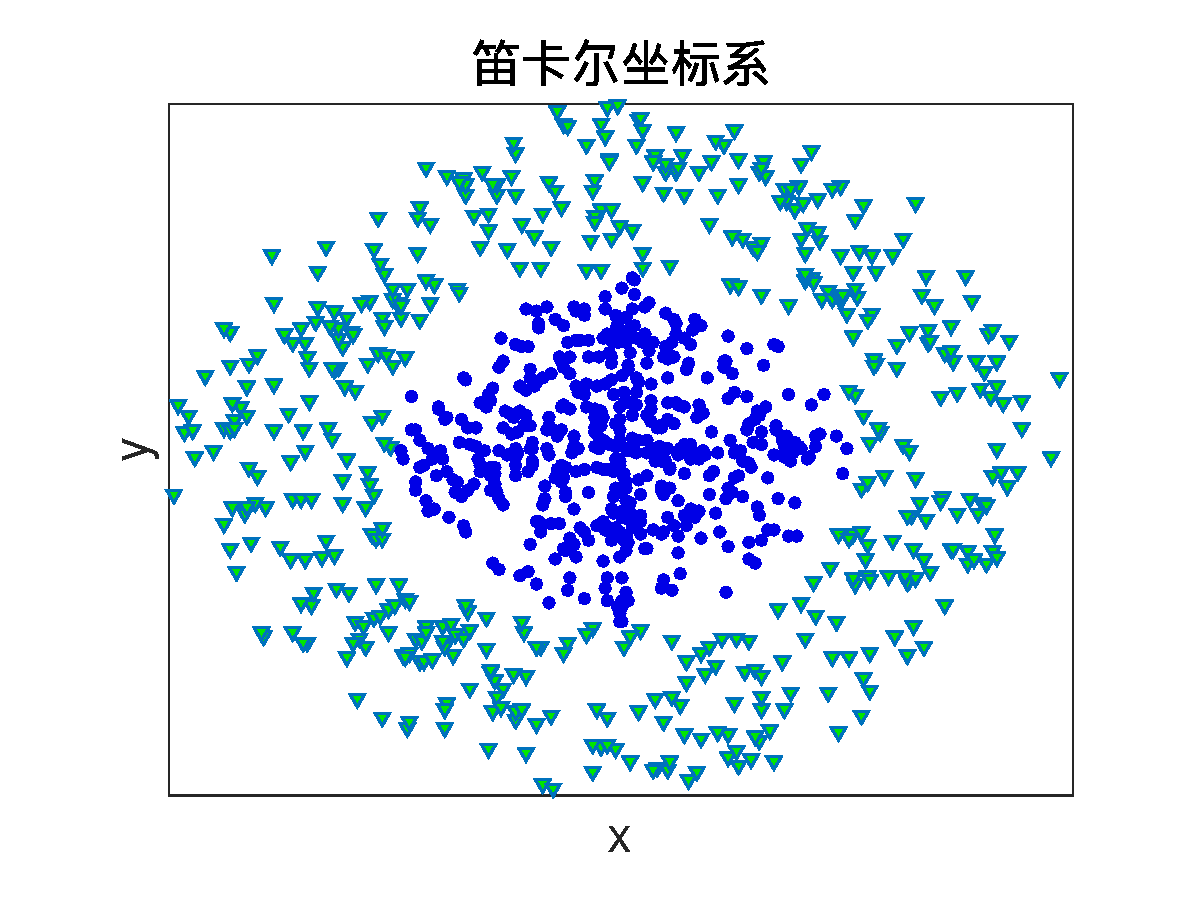
\includegraphics[width=0.45\textwidth]{cartesian_scatter}
  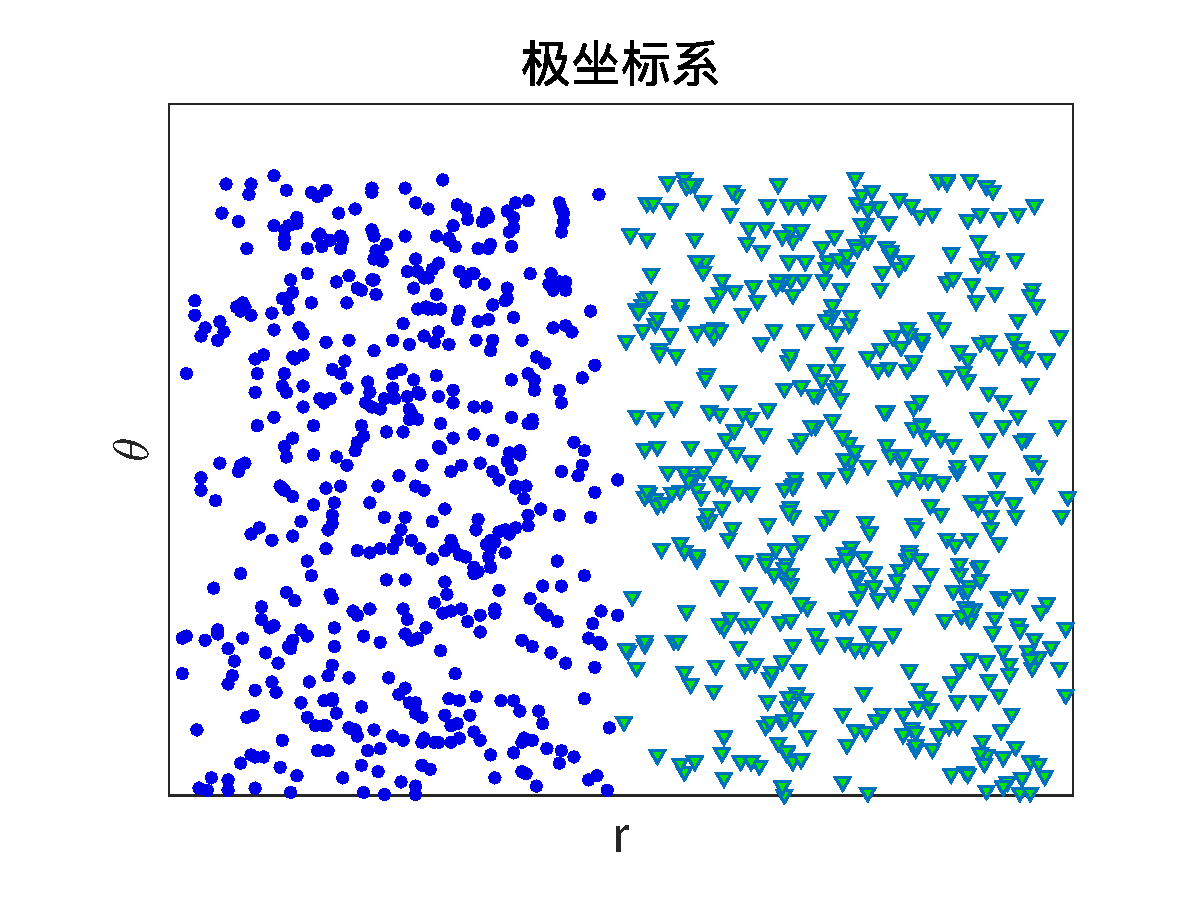
\includegraphics[width=0.45\textwidth]{polar_scatter}
  \caption{不同\gls*{representations}的例子:假设我们想要在一幅散点图中画一条线来
    区分两种数据。在左边的图中,我们使用笛卡尔坐标系描述一些数据,而这个任务是不
    可能的。在右边的图中,我们用极坐标描述一些数据,这个任务就变得很容易用一条竖
    线来解决。这个图由 David Warde-Farley 协助生
    成。\label{fig:different_representations}}
\end{figure}

这个问题的一个解决方法是使用\gls*{ml}来探索不只是从\gls*{representations}到输出的
映射,还有\gls*{representations}本身。这个方法被称为\emph{\gls{rep-learning}}。学
习过的\gls*{representations}往往会导致比手工设计的\gls*{representations}更好的性
能。它们还允许 AI 系统以最少的人为干预来快速地适应新的任务。一
个\gls*{rep-learning}算法可以在几分钟内为一个简单的任务发现一个很好的特征集,或者
对一个复杂的任务,需要几个小时到几个月。手动为一个复杂的任务设计特征需要大量的时
间和人力;它可能耗费整个研究社区几十年的时间。

一个\gls*{rep-learning}算法的典型例子是\emph{\gls{autoencoder}}。一
个\gls*{autoencoder}由一个\emph{\gls{encoder}}\,和一个\emph{\gls{decoder}}\,组
成,\gls*{encoder}将输入数据转换为不同形式的表征,\gls*{decoder}将新的表征转换回
原始格式。\gls*{autoencoder}被训练成当一个输入进
过\gls*{encoder}然后\gls*{decoder}时保存尽可能多的信息,但也被训练使得新的表征有
各种很好的特性。不同种类的\gls*{autoencoder}的目的是获得不同性质的特性。

当为了学习特征而设计特征或算法时,我们的目标通常是分离能解释被观察数据的%
\emph{\gls{fov}}。在这种背景下,我们用单词``因素''来简单指不同的影响来源;这些因
素通常不是通过乘法组合。这样的因素通常不是能直接观察得到量。相反,它们可能存在于
影响到可观察量的物理世界中不可观察的对象或者不可观察的自然力。它们也可能存在于人
类大脑中的构思,这些构思提供有用的精简解释或推断所观察数据的成因。它们可以被认为
是概念或抽象,帮助我们理解数据中的丰富的变化。当分析一个语音记录时,\gls*{fov}包
括说话人的年龄、性别、口音和他们所说的话。当分析一辆汽车的图像时,\gls*{fov}包括
汽车的位置,汽车的颜色,和太阳的角度和亮度。

在许多现实世界的\gls*{ai}应用中的一个主要困难是,许多\gls*{fov}影响每一个我们能够
观察到的数据。在一辆红色汽车的图像中的单个像素在夜间可能非常接近黑色。汽车轮廓的
形状取决于视角。大多数应用程序都需要我们去\textbf{理清}\gls*{fov}并丢弃我们不在乎
的那些。

当然,从原始数据中提取这样的高层、抽象的特征是很困难的。许多这些\gls*{fov},如一
个说话人的口音,只能通过使用复杂的,几乎是人类水平的对数据的理解来识别。当获取一
个解决原始问题的表征相当困难,初看上去,\gls*{rep-learning}似乎不能帮助我们。

\emph{\gls{dl}}\,通过引入以其它更简单的\gls*{representations}的形式所表示的%s
\gls*{representations},来解决这个\gls*{rep-learning}中的核心问题。\gls*{dl}允许
计算机从更简单的概念中构建出复杂的概念。
图~\ref{fig:illustration_of_a_deep_learning_model} 显示了一个\gls*{dl}系统如何能
够通过结合更简单的概念~——~例如角点和轮廓,这些相应地以边缘的形式定义~——~表示一幅
人像的概念。



\begin{figure}[h]
  \centering
  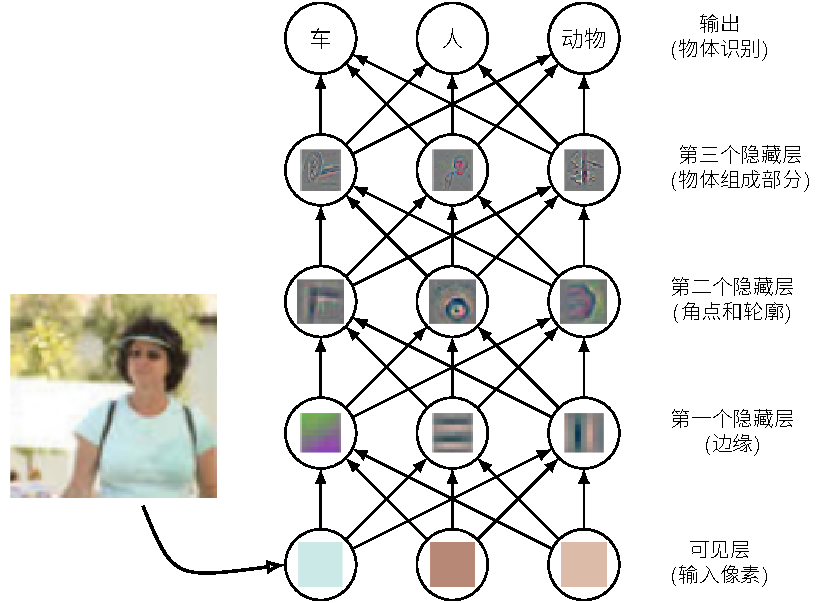
\includegraphics{illustration_of_a_deep_learning_model}
  \caption{一个\gls*{dl}模型的举例。理解原始的传递感觉的输入数据~——~例如这幅表示
    为像素值集合的图像~——~对一台计算机来说是困难的。从一系列像素到一个物体识别的
    特征映射是非常复杂的。学习或评估这个映射,如果直接处理似乎是无法克服
    的。\gls*{dl}通过打破所需的复杂的映射到一系列嵌套的简单的映射~——~每一个由模型
    的一个不同的层描述~——~解决了这个困难。输入被呈现于\textbf{可见层},之所以这样
    命名,是因为它包含了我们能够观察到的变量。然后,是一系列\textbf{隐藏层},从图
    像中提取越来越抽象的功能。这些层被称为``隐藏'',因为他们的值没有在数据中给出;
    相反,模型必须确定哪些概念有助于解释所观察数据的关系。这里的图像是由每一个隐
    藏单元表示的某类特征的可视化处理。给定像素,第一层可以很容易地通过比较相邻像
    素的亮度识别边缘。由于第一个隐藏层对边缘的描述,第二个隐藏层可以很容易地搜索
    的角点和扩展的轮廓,它们可识别为边缘的集合。鉴于第二个隐藏层以角点和轮廓形式
    的图像描述,第三个隐藏层可以通过找出特定的轮廓和角点的集合,检测到整个特定物
    体的组成部分。最后,这个包含有物体组成部分形式的图像描述,可以用来识别图像中
    呈现的物体。这些图像在得到\citet{ZeilerFergus14}许可后重新生
    成。\label{fig:illustration_of_a_deep_learning_model}}
\end{figure}

这一\gls*{dl}模型的典型示例即是前馈深度网络或者\emph{\gls{mlp}}\,(MLP)。一
个\gls*{mlp}仅仅是一个数学函数,映射一系列输入值到输出值。这一函数是由许多更简单
的函数组合而成。你可以把每一个不同数学函数的应用看作提供一个新的输入的表征。

学习正确的数据表征的想法提供了\gls*{dl}上的一个观点。\gls*{dl}的另一个观点是,深
度允许计算机学习一个多步骤的计算机程序。每一层的表征可以被认为是在并行地执行了其
它一组指令后的计算机内存的状态。具有更大深度的网络可以在序列中执行更多的指令。顺
序指令提供了很大的能力,因为以后的指令可以参考前期指令的结果。根据\gls*{dl}的这个
观点,一层的激活中并不是所有的信息必须编码解释输入的\gls*{fov}。表征还存储状态信
息,有助于执行一个可以使输入有意义的程序。这个状态信息可以类似于一个传统的计算机
程序中的计数器或指针。它与输入的具体内容无关,但它帮助模型组织它的处理。

有两种主要的方法来衡量一个模型的深度。第一种观点基于为了评估整个架构必须执行的顺
序指令的数量。我们可以把这看做经过一个流程图的最长路径的长度,这个流程图描述了给
定每个模型的输入如何计算它的输出。正如两个相同的计算机程序会有不同的长度~——~取决
于这个程序是用哪个语言编写的,相同的功能被画成不同深度的流程图~——~取决于允许哪个
功能作为流程图中的单独的步骤。图~\ref{fig:computational_graphs} 说明了这种语言的
选择如何对同一架构给出两个不同的衡量。

\begin{figure}[h]
  \centering
  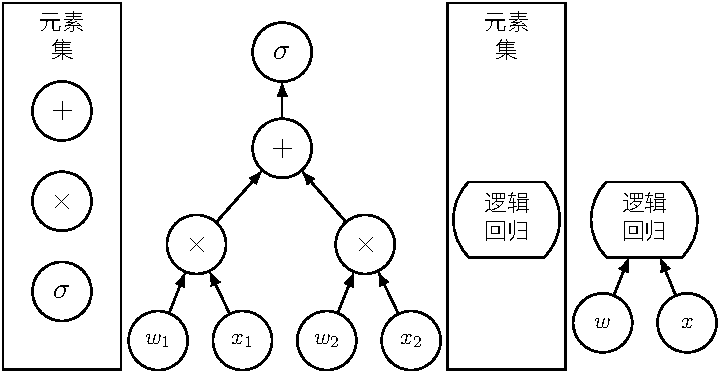
\includegraphics{computational_graphs}
  \caption{将一个输入映射为一个输出的运算图示例,其中每个节点实行一个操作。深度是
    从输入到输出的最长路径长度,但是依赖于构建一个可能的运算步骤的定义。在这些图
    中描绘的运算是一个逻辑回归模型的输出,$\sigma(w^Tx)$,其中 $\sigma$ 是逻辑 S
    型函数。如果我们使用加法、乘法和逻辑 S 型作为我们的计算机语言的元素,那么这个
    模型深度为 3。如果我们把逻辑回归本身看做一个元素,那么这个模型深度
    为 1。\label{fig:computational_graphs}}
\end{figure}

另一个在深度概率模型中使用的方法,并不将一个模型的深度看做运算图形的深度,而是描
述概念间如何彼此相互关联的图形深度。在这种情况下,运算流程图~——~其中需要计算每个
概念的表征~——~的深度,可能比这些概念自身的图形要深得多。这是因为系统在更小概念上
的理解,在给出关于更复杂概念的信息时,能够被改进。例如,一个正在观察一张人脸图
像~——~其中一只眼睛被阴影遮住~——~的 AI 系统,可能起初只看到一个眼睛。在检测到呈现
的是一张人脸后,它能够推断出很可能也有第二只眼睛。在这个情况下,概念图仅包含两
层~——~一层针对眼睛,一层针对人脸~——~但是如果我们改进对每个概念的估算,给予另外
的 $n$ 次,那么运算图形包含有 $2n$ 层。

由于这两种观点~——~运算图形的深度,或者概率模型图形的深度~——~中哪一个最有实质作用
并不总是很清晰,并且因为不同的人选择不同的最小元素的集合来构造他们的图形,对一个
架构的深度来说没有一个唯一正确的值,就像对一个计算机程序的长度来说没有一个唯一正
确的值。同样关于一个模型需要有多少深度才有资格被评为``深的''也没有一个共识。然
而,\gls*{dl}能够可靠地被用于研究那些比传统\gls*{ml}涉及到由更多通过学习获得的功
能或概念构成的模型。

总结来说,\gls*{dl},这本书的主题,是一种 AI 方法。特别地,它是一种\gls*{ml}类型,
一种允许计算机系统随着经验和数据改进的技术。按照本书的作者们,\gls*{ml}是构建能够
在复杂的、真实的环境中运行的 AI 系统的唯一切实可行的方法。\gls*{dl}是一种特殊
的\gls*{ml},通过学习将世界表示成嵌套的概念层次~——~每个概念由相关的更简单的概念定
义,而更抽象的\gls*{representations}以更少抽象的\gls*{representations}形式计
算~——~实现了强大的能力和灵活性。图~\ref{fig:venn_diagram} 阐明了这些不同 AI 学科
之间的关系。图~\ref{fig:different_ai_disciplines} 给出了每一个如何工作的高层次原
理图。

\begin{figure}[h]
  \centering
  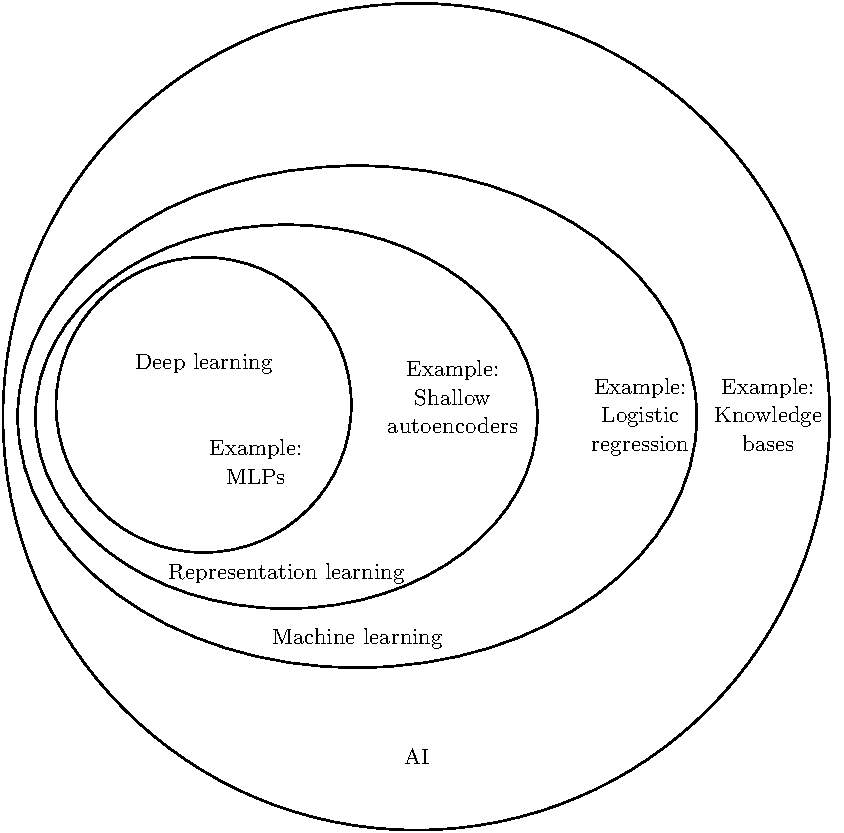
\includegraphics{venn_diagram}
  \caption{一个维恩图,显示\gls*{dl}如何是\gls*{rep-learning}的一个类型,其相应地
    是\gls*{ml}的一个类型,\gls*{ml}是许多但不是全部 AI 的方法。每个维恩图的一个
    部分包含有一个 AI 技术的示例。\label{fig:venn_diagram}}
\end{figure}

\begin{figure}[h]
  \centering
  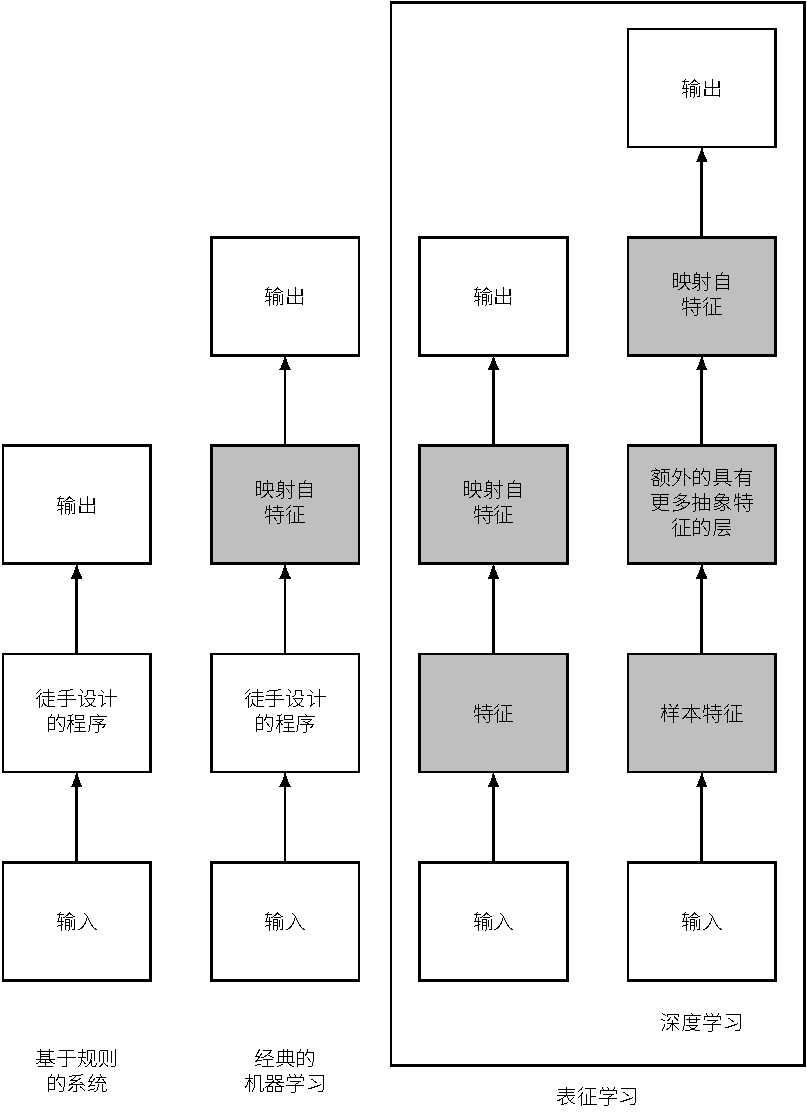
\includegraphics{different_ai_disciplines}
  \caption{显示不同的 AI 学科中的一个 AI 系统中不同的部分如何中相互联系的流程图。
    着色的方框表明这些组件能够从数据中学
    习。\label{fig:different_ai_disciplines}}
\end{figure}

\section{谁应该读这本书?}
\label{sec:who_should_read_this_book}

这本书对各种读者都会有用,但我们心怀两个主要的受众来写它。一个目标受众是正在学习
\gls*{ml}的大学学生(本科生或研究生),包括那些开启职业生涯于\gls*{dl}和
\gls*{ai}研究的学生。另一个目标受众是没有\gls*{ml}或统计背景的软件工程师,但是想
要快速获得并在他们的产品或平台上开始使用\gls*{dl}。\gls*{dl}已经被证明在许多软件
学科中是有用的,包括计算机视觉、语音处理、自然语言处理、机器人学、生物信息学和化
学、视频游戏、搜索引擎、在线广告和金融。

这本书被组织为三个部分,以便适应于各种读者。第\hyperref[part_basics]{一}部分介绍
基础的数学工具和\gls*{ml}概念。第\hyperref[part_practical]{二}部分描述大部分已经
认可的\gls*{dl}算法,它们是基本上已经被解决的技术。第\hyperref[part_research]{三}部
分描述更多推测性的概念,它们被广泛认为在未来的\gls*{dl}中是重要的。

读者可以按照他们的兴趣和背景随意跳过那些不相关的部分。例如,熟悉线性代数,概率,
和基本的\gls*{ml}概念的读者可以跳过第\hyperref[part_basics]{一}部分,而只想实现
一个可工作的系统的读者不需要阅读第\hyperref[part_practical]{二}部分之外的内容。
为了帮助选择哪些章节阅读,图 1.6 提供了一个流程图,显示了该书的高层次组织。

\begin{figure}[h]
  \centering
  \begin{tikzpicture}[
      base/.style={rectangle,draw,thick,inner sep=0pt,font=\small},
      chap/.style={base,minimum width=20mm,minimum height=10mm}
    ]

    \node(c1) [chap] {1.介绍};
  \end{tikzpicture}
  \caption{The high-level organization of the book. An arrow from one chapter to
    another indicates that the former chapter is prerequisite material for
    understanding the latter\label{book_organization}}
\end{figure}

我们假设所有的读者都来自计算机科学背景。

\section{深度学习的历史趋势}



\subsection{不断增长的模型规模}
\label{subsec:increasing_model_sizes}
